\documentclass{beamer}
% \bibliography{references.bib}
\usepackage{amsmath}
\usepackage{amssymb}
\usepackage{braket}
\usepackage[backend=biber, style=alphabetic]{biblatex}
\bibliography{references.bib}
\usepackage{tikz}
\usepackage{xcolor}
\usepackage{bm}
\usepackage{dsfont}

\usepackage[compat=0.6]{yquant}
\usetheme{Madrid}
\usepackage{algorithm}
\usepackage{algpseudocode}
\usepackage{nicematrix}
\usepackage{pgfplots}
\pgfplotsset{compat=1.18}

\usetikzlibrary{fit,quotes}
\usetikzlibrary{trees}


\pgfdeclareshape{yquant-multictrlshape}{
   \inheritsavedanchors[from=yquant-circle]%
   \foreach \anc in {center, north, north east, east, south east, south, south west, west, north west} {%
      \inheritanchor[from=yquant-circle]{\anc}%
   }%
   \inheritanchorborder[from=yquant-circle]%
   \backgroundpath{%
      \pgfpathmoveto{\pgfqpoint{-0.707107\dimexpr\xradius\relax}{-0.707107\dimexpr\yradius\relax}}%
      \pgfpathlineto{\pgfqpoint{0.707107\dimexpr\xradius\relax}{0.707107\dimexpr\yradius\relax}}%
      \pgfpathellipse{\pgfpointorigin}%
                     {\pgfqpoint{\xradius}{0pt}}%
                     {\pgfqpoint{0pt}{\yradius}}%
   }%
   \inheritclippath[from=yquant-circle]%
}


\pgfdeclareshape{yquant-varmultictrlshape}{
   \inheritsavedanchors[from=yquant-circle]%
   \foreach \anc in {center, north, north east, east, south east, south, south west, west, north west} {%
      \inheritanchor[from=yquant-circle]{\anc}%
   }%
   \inheritanchorborder[from=yquant-circle]%
   \backgroundpath{%
      \pgfpathmoveto{\pgfqpoint{-0.707107\dimexpr\xradius\relax}{-0.707107\dimexpr\yradius\relax}}%
      \pgfpathlineto{\pgfqpoint{0.707107\dimexpr\xradius\relax}{0.707107\dimexpr\yradius\relax}}%
      \pgfpathellipse{\pgfpointorigin}%
                     {\pgfqpoint{\xradius}{0pt}}%
                     {\pgfqpoint{0pt}{\yradius}}%
   }%
   \behindbackgroundpath{%
      \begin{pgfscope}
         % Shift to the center and move up by 1.2 times the yradius
         \pgftransformshift{\pgfqpoint{0pt}{\dimexpr-1\yradius\relax}}
         % Scale the tilde
         \pgftext[center,base]{\scalebox{1.2}{$\tilde{}$}}
      \end{pgfscope}
   }%
   \inheritclippath[from=yquant-circle]%
}

\yquantset{multictrlpos/.style={every positive control/.style={draw, /yquant/default fill,shape=yquant-multictrlshape,radius=1.05mm}}}

\yquantset{multictrl/.style={every negative control/.style={draw, /yquant/default fill,shape=yquant-multictrlshape,radius=1.05mm}}}
\yquantset{varmultictrl/.style={/yquant/every control/.style={shape=yquant-varmultictrlshape,radius=1.05mm}}}

\yquantset{plusctrl/.style={/yquant/every control/.style={/yquant/operators/every not}, every positive control/.style={}}}


\title[Piecewise QSVT Data Loading]{Quantum state preparation via piecewise QSVT\footfullcite{obrien2024quantumstatepreparationpiecewise}}
\author[O. O'Brien, C. Sünderhauf] % (optional)
{Oliver O'Brien and Christoph Sünderhauf}
\institute{Riverlane}
\date{July 2024}



\begin{document}

\frame{\titlepage}
\section{Motivation}

\section{QSVT}
% \begin{frame}
% \frametitle{Motivation}
% \begin{itemize}
%     \item Exactly preparing an arbitrary quantum state $\ket{\psi}$ is costly, as the circuit must input each unique amplitude $c_x$ via a rotation
%     $$
%     \ket{\psi} =  \sum_{x=0}^{N-1} c_x \ket{x}
%     $$
%     \pause
%     \item \textbf{Idea}: Can we use some compression technique to prepare approximate states more efficiently? 
%     \pause
%     \begin{itemize}
%         \item Yes! If our amplitudes can be \textbf{efficiently} approximated by a polynomial \footfullcite{mcardleQuantumStatePreparation2022}
%     \end{itemize}
% \end{itemize}
% \end{frame}
  \begin{frame}
   \begin{figure}
    \centering

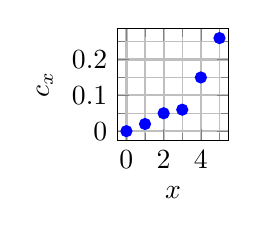
\begin{tikzpicture}
  \begin{axis}[
    xlabel=$x$,
    ylabel=$c_x$,
    grid=both,
    minor tick num=1, % Number of minor ticks per major tick
    major grid style={line width=0.8pt,draw=gray!50},
    width=3cm,
    height=3cm,
    legend style={at={(1,1)},anchor=north east}
  ]
    % Scatter plot points
    \addplot[
      only marks,
      mark=*,
      color=blue,
      mark size=2pt
    ] coordinates {
      (0,0) (1,0.02) (2,0.05) (3,0.06) (4,0.15) (5,0.26)
    };
    % \addlegendentry{Data points}
    
    % Polynomial approximation (e.g., quadratic)
    % \addlegendentry{Polynomial approximation}
  \end{axis}
\end{tikzpicture}
\begin{tikzpicture}[overlay]
\draw[->, thick] (0,1.5) -- (1,1.5); % Adjust coordinates as needed
\node at (0.5,1.75) {Approx};
\end{tikzpicture}
\hspace{1cm}
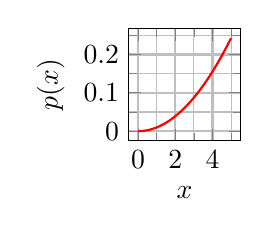
\begin{tikzpicture}
  \begin{axis}[
    xlabel=$x$,
    ylabel=$p(x)$,
    grid=both,
    minor tick num=1, % Number of minor ticks per major tick
    major grid style={line width=0.8pt,draw=gray!50},
    width=3cm,
    height=3cm,
    legend style={at={(1,1)},anchor=north east}
  ]
    % Scatter plot points
    % \addplot[
    %   only marks,
    %   mark=*,
    %   color=blue,
    %   mark size=2pt
    % ] coordinates {
    %   (0,0) (1,1) (2,4) (3,9) (4,16) (5,25)
    % };
    % \addlegendentry{Data points}
    
    % Polynomial approximation (e.g., quadratic)
    \addplot[
      domain=0:5,
      samples=100,
      color=red,
      thick
    ] {0.0097*x^2};
    % \addlegendentry{Polynomial approximation}
  \end{axis}
\end{tikzpicture}
\begin{tikzpicture}[overlay]
\draw[->, thick] (0,1.5) -- (1,1.5); % Adjust coordinates as needed
\node at (0.5,1.75) {QSVT};
\end{tikzpicture}
\hspace{1cm}
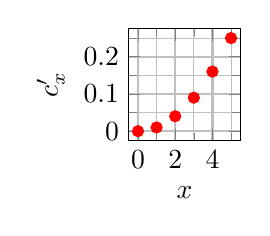
\begin{tikzpicture}
  \begin{axis}[
    xlabel=$x$,
    ylabel=$c'_x$,
    grid=both,
    minor tick num=1, % Number of minor ticks per major tick
    major grid style={line width=0.8pt,draw=gray!50},
    width=3cm,
    height=3cm,
    legend style={at={(1,1)},anchor=north east}
  ]
    % Scatter plot points
    \addplot[
      only marks,
      mark=*,
      color=red,
      mark size=2pt
    ] coordinates {
      (0,0) (1,0.01) (2,0.04) (3,0.09) (4,0.16) (5,0.25)
    };
    % \addlegendentry{Data points}
    
    % Polynomial approximation (e.g., quadratic)
    % \addplot[
    %   domain=0:5,
    %   samples=100,
    %   color=red,
    %   thick
    % ] {0.97*x^2};
    % \addlegendentry{Polynomial approximation}
  \end{axis}
\end{tikzpicture}
\tableofcontents[currentsection]
\end{figure}
\end{frame}
% \begin{frame}
%     \begin{itemize}
%         \item Quantum Signal Processing: 
%         $$
%         S(\phi_0) \prod_{k=1}^{d} U(a) S(\phi_k) = \begin{pmatrix} P(a) & \ast \\ \ast & \ast \end{pmatrix}
%         $$
%         $$
%         U(a) = \begin{pmatrix} a & \sqrt{1-a^2} \\ \sqrt{1-a^2} & -a \end{pmatrix}
%         $$
%         $$
%         S(\phi) =\begin{pmatrix} e^{i\phi} & 0 \\ 0 & e^{-i\phi} \end{pmatrix}
%         $$
%         \item Quantum Singular Value Transformation:
%         $$
%         U(A) = \begin{pmatrix} A & \sqrt{1-AA^{\dagger}} \\ \sqrt{1-AA^{\dagger}} & -A \end{pmatrix}
%         $$
%         $$
%         S(\phi) =\begin{pmatrix} e^{i\phi}\mathds{1} & \bm 0 \\ \bm 0 & e^{-i\phi} \mathds{1} \end{pmatrix}
%         $$
%     \end{itemize}
% \end{frame}
\begin{frame}
\begin{itemize}
    \item Definite parity QSVT circuit with 2 steps:
    \begin{equation*}
\begin{tikzpicture}
\begin{yquant}
qubit {QSVT flag} flag1;
qubit {BE flag} flags;
qubit {$x$} n;


["north:$N$" {font=\protect\footnotesize, inner sep=0pt}]
slash n;

% h flag1;

[multictrl]
box {$U$} (flags, n) ;
cnot flag1 ~ flags;


box {$R_z(\phi_{0})$} flag1;
cnot flag1 ~ flags;

[multictrl]
box {$U^\dag$} (flags, n) ;
cnot flag1 ~ flags;


box {$R_z(\phi_{1})$} flag1;
cnot flag1 ~ flags;
% h flag1;

\end{yquant}
\end{tikzpicture}
\end{equation*}
\item Circuit encodes: $$
        \begin{pmatrix} P(A) & \ast \\ \ast & \ast \end{pmatrix}
        $$
    \item Phase factors $\phi$ describe polynomial $P$
    \item Block encoding $U$ describes matrix A 
    $$
        U(A) = \begin{pmatrix} A & \sqrt{1-AA^{\dagger}} \\ \sqrt{1-AA^{\dagger}} & -A \end{pmatrix}
        $$
\end{itemize}
\end{frame}
\begin{frame}
\begin{itemize}
\item QSVT transforms the singular values of a block encoding by a given polynomial $p$
\item Given a linear diagonal block encoding QSVT produces a diagonal block encoding of equispaced samples from a given polynomial
\begin{equation*}
U = 
\begin{pNiceArray}{ccc|ccc}
  1 & 0 &  & \Block{3-3}<\Large>{j_1} &&\\
  0 & \ddots  & 0\\
     & 0 & -\frac{N-2}{N}\\
  \hline
  \Block{3-3}<\Large>{j_2} &&& \Block{3-3}<\Large>{j_3} &&\\
  &&&\\
  &&&
\end{pNiceArray}\rightarrow
\begin{pNiceArray}{ccc|ccc}
p\left(1 \right) & 0 &  & \Block{3-3}<\Large>{j_4} &&\\
0 & \ddots & 0\\
 & 0 & p(-\frac{N-2}{N})\\
  \hline
  \Block{3-3}<\Large>{j_5} &&& \Block{3-3}<\Large>{j_6} &&\\
  &&&\\
  &&&
\end{pNiceArray} = V
\end{equation*}
\item $V$ can be converted into a state by applying to a uniform superposition and then applying amplitude amplification
\end{itemize}
\end{frame}
% \begin{frame}
% \begin{itemize}
%     \item Indefinite parity QSVT circuit with 2 steps:
%     \begin{equation*}
% \begin{tikzpicture}
% \begin{yquant}
% qubit {QSVT flag} flag1;
% qubit {BE flag} flags;
% qubit {$x$} n;


% ["north:$N$" {font=\protect\footnotesize, inner sep=0pt}]
% slash n;

% h flag1;

% [multictrl]
% box {$U$} (flags, n) | flag1 ;
% cnot flag1 ~ flags;


% box {$R_z(\phi_{0})$} flag1;
% cnot flag1 ~ flags;

% [multictrl]
% box {$U^\dag$} (flags, n) | flag1 ;
% cnot flag1 ~ flags;


% box {$R_z(\phi_{1})$} flag1;
% cnot flag1 ~ flags;

% h flag1;
% \end{yquant}
% \end{tikzpicture}
% \pause
% \end{equation*}
% \item QSVT step is repeated $2d$ times to implement $d$ degree polynomial
% \pause
% \item We require $U$ to be a linear diagonal block encoding such as:
% \begin{equation*}
% \begin{tikzpicture}
% \begin{yquant}
% qubit {QSVT flag} flag2;
% qubit {BE flag} flag1;
% qubit {anc} flags;
% qubit {$\ket{x}$} block;

% ["north:$N$" {font=\protect\footnotesize, inner sep=0pt}]
% slash block;

% ["north:$N$" {font=\protect\footnotesize, inner sep=0pt}]
% slash flags;


% [multictrl]
% box {$U$} (flag1, flags, block)|  flag2;

% text {$=$} (-);

% ["north:$N$" {font=\protect\footnotesize, inner sep=0pt}]
% slash block;

% ["north:$N$" {font=\protect\footnotesize, inner sep=0pt}]
% slash flags;


% h flags;

% align -;
% text {$\ket{0}$} flag1;
% text {$\ket{k}$} flags;
% text {$\ket{x}$} block;

% [multictrl]
% box {high bit\\ add} (block, flags, flag1) |  flag2;

% text {$\ket{k }$} flags;
% text {$\ket{x }$} block;
% text {$\ket{(k+x)\ge 2^{N}}$} flag1;

% x flag1;
% h flags;
% \end{yquant}
% \end{tikzpicture}
% \end{equation*}
% \end{itemize}
% \end{frame}
\section{Piecewise QSVT}
  \begin{frame}
   \begin{figure}
    \centering

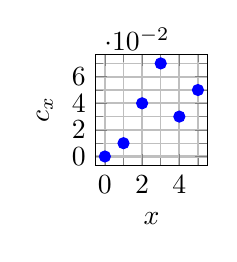
\begin{tikzpicture}
  \begin{axis}[
    xlabel=$x$,
    ylabel=$c_x$,
    grid=both,
    minor tick num=1, % Number of minor ticks per major tick
    major grid style={line width=0.8pt,draw=gray!50},
    width=3cm,
    height=3cm,
    legend style={at={(1,1)},anchor=north east}
  ]
    % Scatter plot points
    \addplot[
      only marks,
      mark=*,
      color=blue,
      mark size=2pt
    ] coordinates {
      (0,0) (1,0.01) (2,0.04) (3,0.07) (4,0.03) (5,0.05)
    };
    % \addlegendentry{Data points}
    
    % Polynomial approximation (e.g., quadratic)
    % \addlegendentry{Polynomial approximation}
  \end{axis}
\end{tikzpicture}
\begin{tikzpicture}[overlay]
\draw[->, thick] (0,1.5) -- (1,1.5); % Adjust coordinates as needed
\node at (0.5,1.75) {Approx};
\end{tikzpicture}
\hspace{1cm}
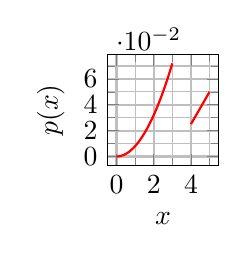
\begin{tikzpicture}
  \begin{axis}[
    xlabel=$x$,
    ylabel=$p(x)$,
    grid=both,
    minor tick num=1, % Number of minor ticks per major tick
    major grid style={line width=0.8pt,draw=gray!50},
    width=3cm,
    height=3cm,
    legend style={at={(1,1)},anchor=north east}
  ]
    % Scatter plot points
    % \addplot[
    %   only marks,
    %   mark=*,
    %   color=blue,
    %   mark size=2pt
    % ] coordinates {
    %   (0,0) (1,1) (2,4) (3,9) (4,16) (5,25)
    % };
    % \addlegendentry{Data points}
    
    % Polynomial approximation (e.g., quadratic)
    \addplot[
      domain=0:3,
      samples=100,
      color=red,
      thick
    ] {0.008*x^2};
    \addplot[
      domain=4:5,
      samples=100,
      color=red,
      thick
    ] {0.025*(x-3)};
    % \addlegendentry{Polynomial approximation}
  \end{axis}
\end{tikzpicture}
\begin{tikzpicture}[overlay]
\draw[->, thick] (0,1.5) -- (1,1.5); % Adjust coordinates as needed
\node at (0.5,1.75) {QSVT};
\end{tikzpicture}
\hspace{1cm}
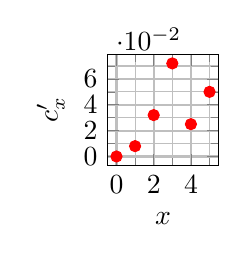
\begin{tikzpicture}
  \begin{axis}[
    xlabel=$x$,
    ylabel=$c'_x$,
    grid=both,
    minor tick num=1, % Number of minor ticks per major tick
    major grid style={line width=0.8pt,draw=gray!50},
    width=3cm,
    height=3cm,
    legend style={at={(1,1)},anchor=north east}
  ]
    % Scatter plot points
    \addplot[
      only marks,
      mark=*,
      color=red,
      mark size=2pt
    ] coordinates {
      (0,0) (1,0.008) (2,0.032) (3,0.072) (4,0.025) (5,0.05)
    };
    % \addlegendentry{Data points}
    
    % Polynomial approximation (e.g., quadratic)
    % \addplot[
    %   domain=0:5,
    %   samples=100,
    %   color=red,
    %   thick
    % ] {0.97*x^2};
    % \addlegendentry{Polynomial approximation}
  \end{axis}
\end{tikzpicture}
\tableofcontents[currentsection]
\end{figure}
\end{frame}
\begin{frame}
\begin{itemize}
\item To perform piecewise QSVT we perform a different $d$-degree polynomial transformations $p_{s}$ on $S$ different $L_{s}$ long sections of the block encoding, and each section of the block encoding is linear between 1 and -1
\end{itemize}
\begin{equation*}
% \begin{pNiceArray}{ccccccc|cc}
%   \frac{1}{L_1} &  & && & & & \Block{7-2}<\Large>{j_1} &\\
%    & \ddots  &  & & && \\
%      &  & 1 & & & &\\
%      & & & \ddots & & & \\
%      & & && \frac{1}{L_m}&  & \\
%      & & && &\ddots &  \\
%      & & & && & 1 \\
%   \hline
%   \Block{2-7}<\Large>{j_2} &&&&&& & \Block{2-2}<\Large>{j_3} &\\
%   &&&&&\\
% \end{pNiceArray}\rightarrow
\begin{pNiceArray}{ccccccc|cc}
  p_0\left(1\right) &  & && & & & \Block{7-2}<\Large>{j_1} &\\
   & \ddots  &  & & && \\
     &  & p_0\left(-\frac{L_0-2}{L_0}\right) & & & &\\
     & & & \ddots & & & \\
     & & && p_{S-1}\left(1\right)&  & \\
     & & && &\ddots &  \\
     & & & && & p_{S-1}\left(-\frac{L_{S-1}-2}{L_{S-1}}\right) \\
  \hline
  \Block{2-7}<\Large>{j_2} &&&&&& & \Block{2-2}<\Large>{j_3} &\\
  &&&&&\\
\end{pNiceArray}
\end{equation*}

\end{frame}
\begin{frame}
\begin{itemize}
    \item The block encoding of $S$ linear sections between 1 and -1 is given by:

\begin{equation*}
\begin{tikzpicture}[scale=0.8]
\begin{yquant}

% qubit {parity bit} hb;

qubit {flag} flag1;
qubit {flags} flags;
qubit {$\ket{x}$} block;
qubit {control} flag2;

["north:$n$" {font=\protect\footnotesize, inner sep=0pt}]
slash block;

["north:$l_{max}$" {font=\protect\footnotesize, inner sep=0pt}]
slash flags;


[multictrl]
box {$U$} ( flag1, flags, block)|  flag2 ;

text {$=$} (-);
slash block;
slash flags;


x flag1;
h flag1;

h flags;


align -;
text {$\frac{(-1)^a}{\sqrt{2}}\ket{a}$} flag1;
text {$\ket{k}$} flags;
text {$\ket{x}$} block;
% text {$\ket{+}$} hb;

[multictrl]
box {CC} (flag1) |  flag2 ~ flags, block ;

% z hb;



text {$\ket{k }$} flags;
text {$\ket{x }$} block;
text {$\frac{(-1)^a}{\sqrt{2}}\ket{a \oplus (k_{l_{s_x}}+x_{l_{s_x}}\ge 2^{l_{s_x}}) }$} flag1;

h flag1;
x flag1;

% cnot flag1 | hb;
% h hb;
h flags;
\end{yquant}
\end{tikzpicture}
\end{equation*}
\item $2^{l_{s_x}}$ is the length of the section $s_x$ that $x$ belongs to
\item $k_{l_{s_x}}$ and $x_{l_{s_x}}$ are the least significant $l_{s_x}$ bits of $k$ and $x$ respectively:
    $$
    k_{l_{s_x}} = k \mod 2^{l_{s_x}}
$$
\item $x$-th diagonal entry of block encoding is $ \frac{2^{l_{s_x}} - 2x_{l_{s_x}}}{2^{l_{s_x}}}$
\item Only costs $4l_{max} + 11S -4$ T gates
    \end{itemize}
\end{frame}
\begin{frame}
\begin{itemize}
    \item Piecewise indefinite-parity QSVT circuit:
\begin{equation*}
\begin{tikzpicture}[scale=0.8]
\begin{yquant}
qubit {QSVT flag} flag1;

qubit {BE flags} f;
qubit {BE flags} flags;
qubit {$x$} n;

["north:$l_{max}$" {font=\protect\footnotesize, inner sep=0pt}]
slash flags;

["north:$n$" {font=\protect\footnotesize, inner sep=0pt}]
slash n;




[multictrl]
box {$R_X(\phi_{0,s_{x}})$} flag1 ~ n;

[operator style={/yquant/every negative control}]
phase {} flags ~  f, flag1;
[multictrlpos]
box {$U$} (flags,f, n)  ~ flag1;


[multictrl]
box {$R_X(\phi_{1,s_{x}})$} flag1 ~ n;


[multictrl]
box {$U$} (flags,f, n) | flag1 ;

[operator style={/yquant/every positive control}]
phase {} flag1  ~ flags, f;
[multictrl]
box {$R_X(\phi_{2,s_{x}})$} flag1 ~ n;


\end{yquant}
\end{tikzpicture}
\end{equation*}

    \item Magic ingredient is variable unary iteration \cite{Sanders_2020}
        % \item Works by ignoring bits of x:
        \small
    \[
    \begin{aligned}
        &\left.
        \begin{aligned}
        &000 \\
        \end{aligned}
        \right\} \quad s_x=0 \quad l_x = 0&\\
        &\left.
        \begin{aligned}
        &001 \\
        \end{aligned}
        \right\} \quad s_x=1 \quad l_x = 0&\\
        &\left.
        \begin{aligned}
        &01{\textcolor{lightgray}{0}} \\
        &01{\textcolor{lightgray}{1}} 
        \end{aligned}
        \right\} \quad s_x=2 \quad l_x = 1&\\
        &\left.\begin{aligned}
            &1{\textcolor{lightgray}{00}} \\
            &1{\textcolor{lightgray}{01}} \\
            &1{\textcolor{lightgray}{10}} \\
            &1{\textcolor{lightgray}{11}}
        \end{aligned}
        \right\} \quad s_x=3 \quad l_x = 2&\\
    \end{aligned}
    \]
    \normalsize
    \par\noindent
    \item Requires only $4dS$ rotation gates and $2d$ controlled $U$

    
\end{itemize}
\end{frame}
% \begin{frame}
%    \begin{figure}[t]
% \centering
%   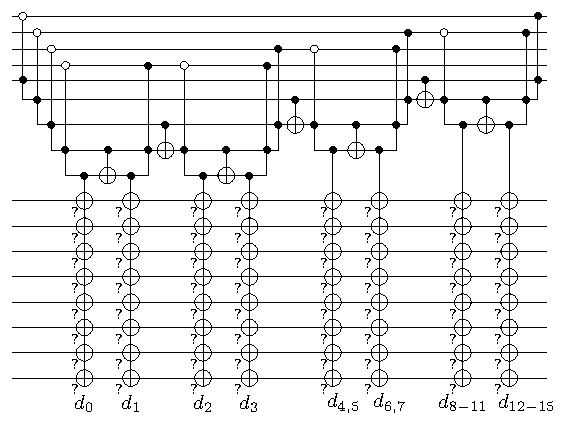
\includegraphics{Qrom.pdf}
%   \caption{Variable unary iteration.\footfullcite{Sanders_2020}}
% \end{figure}
% \end{frame}
% \begin{frame}{Limitations}
% \begin{itemize}
%     \item Variable QROM and the high bit adder only work efficiently on sections that correspond to ignoring bits of $x$
%     \item $|p_i(x)| < 1$ for all $x \in [-1,1]$ and all $i \in \mathbb{Z}_g$
% \end{itemize}
    
% \end{frame}
\section{Piecewise Polynomial Approximations}
\begin{frame}
   \begin{figure}
    \centering

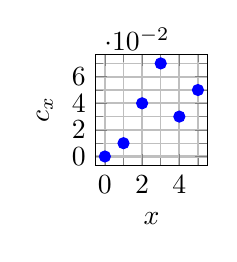
\begin{tikzpicture}
  \begin{axis}[
    xlabel=$x$,
    ylabel=$c_x$,
    grid=both,
    minor tick num=1, % Number of minor ticks per major tick
    major grid style={line width=0.8pt,draw=gray!50},
    width=3cm,
    height=3cm,
    legend style={at={(1,1)},anchor=north east}
  ]
    % Scatter plot points
    \addplot[
      only marks,
      mark=*,
      color=blue,
      mark size=2pt
    ] coordinates {
      (0,0) (1,0.01) (2,0.04) (3,0.07) (4,0.03) (5,0.05)
    };
    % \addlegendentry{Data points}
    
    % Polynomial approximation (e.g., quadratic)
    % \addlegendentry{Polynomial approximation}
  \end{axis}
\end{tikzpicture}
\begin{tikzpicture}[overlay]
\draw[->, thick] (0,1.5) -- (1,1.5); % Adjust coordinates as needed
\node at (0.5,1.75) {Approx};
\end{tikzpicture}
\hspace{1cm}
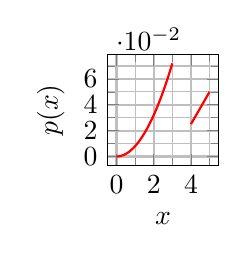
\begin{tikzpicture}
  \begin{axis}[
    xlabel=$x$,
    ylabel=$p(x)$,
    grid=both,
    minor tick num=1, % Number of minor ticks per major tick
    major grid style={line width=0.8pt,draw=gray!50},
    width=3cm,
    height=3cm,
    legend style={at={(1,1)},anchor=north east}
  ]
    % Scatter plot points
    % \addplot[
    %   only marks,
    %   mark=*,
    %   color=blue,
    %   mark size=2pt
    % ] coordinates {
    %   (0,0) (1,1) (2,4) (3,9) (4,16) (5,25)
    % };
    % \addlegendentry{Data points}
    
    % Polynomial approximation (e.g., quadratic)
    \addplot[
      domain=0:3,
      samples=100,
      color=red,
      thick
    ] {0.008*x^2};
    \addplot[
      domain=4:5,
      samples=100,
      color=red,
      thick
    ] {0.025*(x-3)};
    % \addlegendentry{Polynomial approximation}
  \end{axis}
\end{tikzpicture}
\begin{tikzpicture}[overlay]
\draw[->, thick] (0,1.5) -- (1,1.5); % Adjust coordinates as needed
\node at (0.5,1.75) {QSVT};
\end{tikzpicture}
\hspace{1cm}
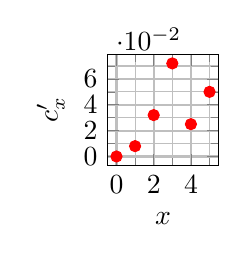
\begin{tikzpicture}
  \begin{axis}[
    xlabel=$x$,
    ylabel=$c'_x$,
    grid=both,
    minor tick num=1, % Number of minor ticks per major tick
    major grid style={line width=0.8pt,draw=gray!50},
    width=3cm,
    height=3cm,
    legend style={at={(1,1)},anchor=north east}
  ]
    % Scatter plot points
    \addplot[
      only marks,
      mark=*,
      color=red,
      mark size=2pt
    ] coordinates {
      (0,0) (1,0.008) (2,0.032) (3,0.072) (4,0.025) (5,0.05)
    };
    % \addlegendentry{Data points}
    
    % Polynomial approximation (e.g., quadratic)
    % \addplot[
    %   domain=0:5,
    %   samples=100,
    %   color=red,
    %   thick
    % ] {0.97*x^2};
    % \addlegendentry{Polynomial approximation}
  \end{axis}
\end{tikzpicture}
\tableofcontents[currentsection]
\end{figure}
\end{frame}
\subsection{$\sqrt{x}$}
% \begin{frame}{$\sqrt{x}$: $O(n\log^2\frac{1}{\epsilon})$ T gates}
% \begin{itemize}
%     \item Explicitly stated as hard for standard QSVT state preparation
%     \item Using Chebyshev polynomials, we can construct a $d$-degree $n$-piecewise polynomial $f_d$ such that:
%     $$
%      |\sqrt{x} - f_{d}(x)| \leq \frac{2}{2+ \sqrt{8}} (3+\sqrt{8})^{-d}
%      $$
%      for $x \in [2^{-n}, 1]$
%     \begin{figure}
%         \centering
%         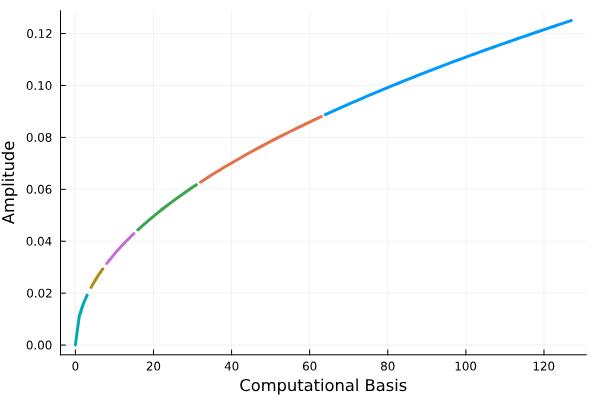
\includegraphics[width=0.5\linewidth]{sqrt_x.png}
%     \end{figure}
%     \item Exponential speed-up over naive state preparation
%     \end{itemize}
% \end{frame}
\subsection{$\log x$}
% \begin{frame}{$\log x$: $O(n^2\log^2 \frac{1}{\epsilon})$ T gates}
% \begin{itemize}
%     \item Using Taylor series expansions we can find $d$-degree $2n$-piecewise polynomial $f_d$ such that:
% $$
% |\frac{1}{\mathcal{N}}\log{x} - f_{d}(x)| \leq  \frac{1}{n(d+1)} 2^{-d-2}.
% $$
% for $x \in [2^{-n+1}, 1]$.
% \end{itemize}
%     \begin{figure}
%         \centering
%         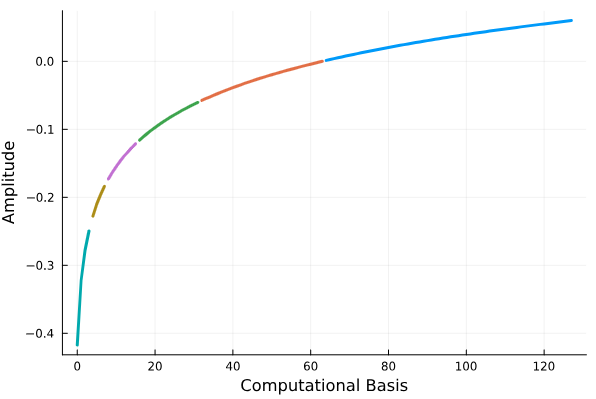
\includegraphics[width=0.5\linewidth]{log_x.png}
%     \end{figure}
% \end{frame}
\subsection{B-Spline window}
\begin{frame}{B-Spline window: $O\left(\max \left(mn,m^2 \log \frac{1}{\epsilon}\right)\right)$ T gates}
    \begin{itemize}
        \item Piecewise polynomial function of degree $m-1$  obtained by $m$-fold self-convolution of the rectangular function
        \begin{equation*}
            m^m \sum_{p=0}^m \frac{(-1)^p}{p!(m-p)!} \left(x - (p - \frac{m}{2})N/m\right)^{m-1} \Theta\left(x - (p - \frac{m}{2})N/m\right)
        \end{equation*}
        \begin{figure}
            \centering
            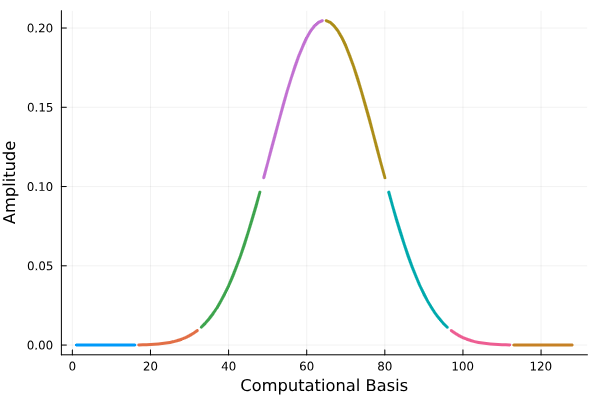
\includegraphics[width=0.5\linewidth]{B-spline.png}\\
            m=8
        \end{figure}
    \end{itemize}
\end{frame}
\begin{frame}{B-Spline window: $O\left(\max \left(mn,m^2 \log \frac{1}{\epsilon}\right)\right)$ T gates}
\begin{itemize}
        \item Useful for boosting Quantum Phase Estimation due to its narrow peak in the Fourier domain:
        \begin{equation*}
            \sqrt{\frac{\pi}{6m}}\left(\frac{\sin \frac{x\pi}{m}}{ \frac{x\pi}{m}}\right)^m
        \end{equation*}
        \begin{block}{Theorem 1}
            To achieve a given probability $\delta$ of measuring energy outside of a given confidence interval $\epsilon$ (when using $O(\log \frac{1}{\delta})$-th B-spline boosted QPE), one must use $O(\log \frac{1}{\epsilon} + \log \log \frac{1}{\delta})$ ancillary qubits.
        \end{block}
        \item This is the same asymptotic scaling as achieved by the Kaiser window
\end{itemize}

\end{frame}
\begin{frame}{B-Spline window: $O\left(\max \left(mn,m^2 \log \frac{1}{\epsilon}\right)\right)$ T gates}
\begin{itemize}
    \item Comparison with cost of implementing Kaiser window using single Taylor series \footfullcite{mcardleQuantumStatePreparation2022}
\end{itemize}
    \begin{figure}
        \centering
        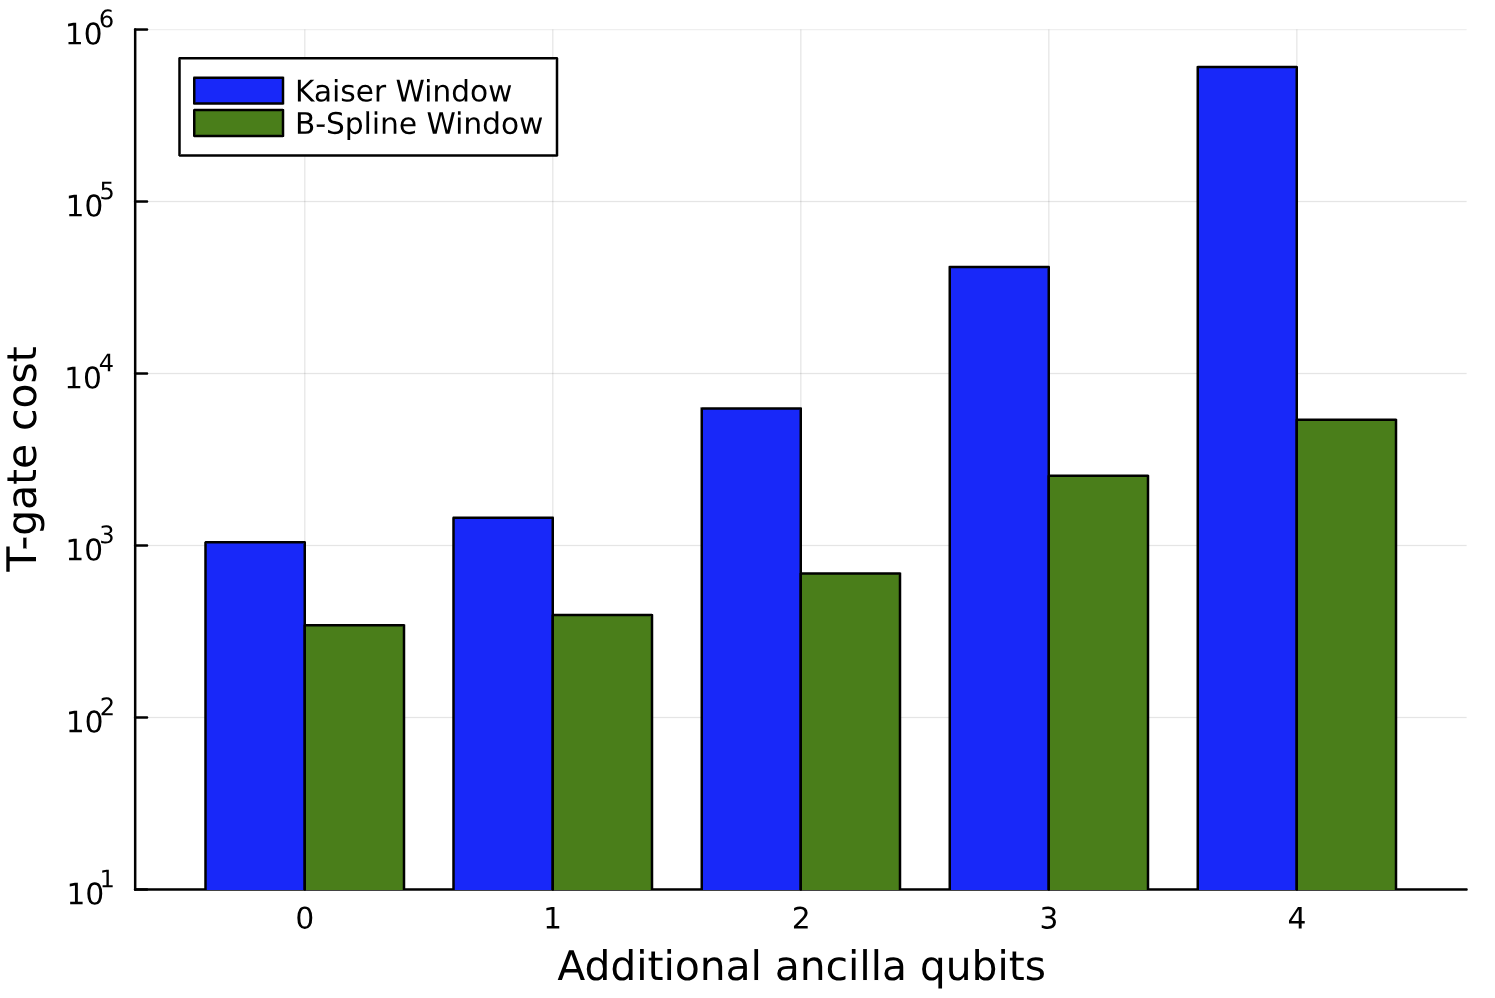
\includegraphics[width=0.45\linewidth]{b-splinevskw.png}
        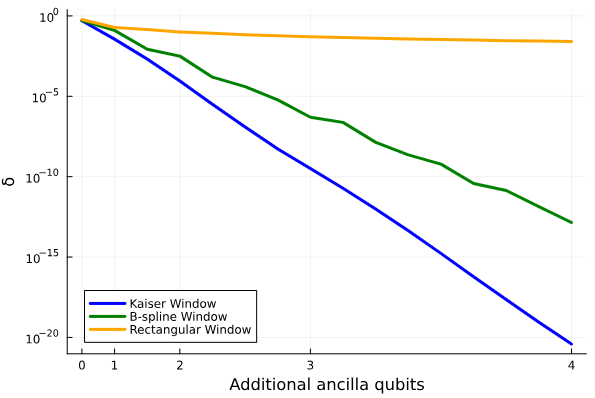
\includegraphics[width=0.45\linewidth]{b-splinevskwanc.png}

    \end{figure}
\end{frame}
\subsection{Generic Algorithm}
\subsection{Your state??}
\begin{frame}{Conclusion}
    \begin{itemize}
        \item Piecewise QSVT can load an $n$-qubit state that can be approximated by a $d$-degree $S$-piece piecewise polynomial with largest piece $2^{l_{max}}$ in $O\left(\max\left(n,dl_{max},dS\log \frac{1}{\epsilon}\right)\right)$ T-gates
        \item Particularly efficient for some identified functions:

           \begin{table}[hbtp]
            \centering
            
            \begin{tabular}{|c|c|}
            \hline Function & T-gate cost\\ \hline\hline
                \rule{0pt}{1.25em}$\sqrt{\frac{x}{N}}$ &  $O\left(n\log^2 \frac{1}{\epsilon}\right)$\\[0.5em] \hline
                \rule{0pt}{1.25em}$\log \frac{x}{N}$ &  $O\left(n^2\log^2 \frac{1}{\epsilon}\right)$ \\[0.5em] \hline
                % $\log x$ & $O(n\log^2 \frac{1}{\epsilon})$ \\ \hline
                \rule{0pt}{1.25em}$m$-th B-spline window & $O\left(\max \left(mn,m^2 \log \frac{1}{\epsilon}\right)\right)$ \\[0.5em] \hline
            \end{tabular}
        \end{table}
        on $n$ qubits with error tolerance $\epsilon$
    \end{itemize}
\end{frame}
\begin{frame}{Implementation of high bit adder}
 \begin{equation*}
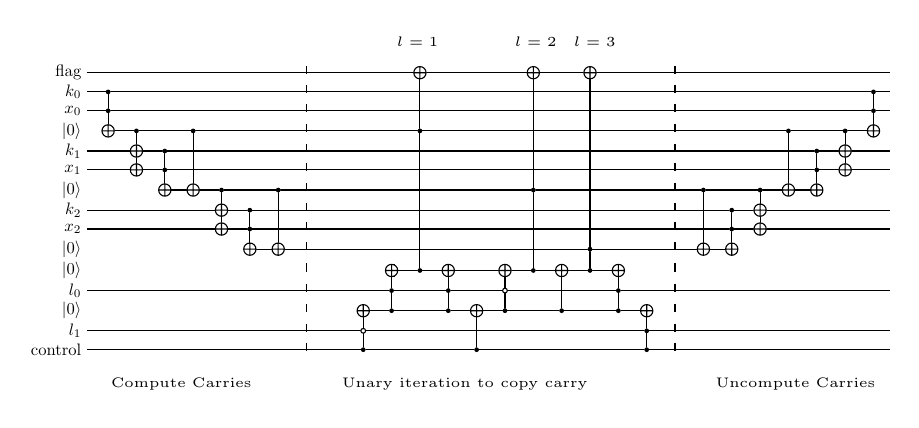
\begin{tikzpicture}[scale=0.6]
\begin{yquant}

qubit {flag} f;



qubit {$k_{0}$} k0;
qubit {$x_{0}$} x0;
qubit {$\ket{0}$} c0;
discard c0;
hspace {-0.5cm} -;

qubit {$k_{1}$} k1;
qubit {$x_{1}$} x1;
qubit {$\ket{0}$} c1;
discard c1;


qubit {$k_{2}$} k2;
qubit {$x_{2}$} x2;
qubit {$\ket{0}$} c2;
discard c2;

qubit {$\ket{0}$} anc1;
discard anc1;
qubit {$l_{0}$} l1;
qubit {$\ket{0}$} anc0;
discard anc0;
qubit {$l_{1}$} l0;



qubit {control} flag;

setstyle {|-, shorten <= 0.25cm} c0;
init {} c0;
cnot c0 | x0, k0;


cnot x1, k1 | c0;

setstyle {|-, shorten <= 0.8cm} c1;
init {} c1;

cnot c1 | k1, x1;
cnot c1 | c0;

cnot x2, k2 | c1;
setstyle {|-, shorten <= 1.85cm} c2;
init {} c2;

cnot c2 | k2, x2;
cnot c2 | c1;


barrier l0, l1, flag, anc0, anc1, x0, k0, x1, k1, x2, k2, c0, c1, c2, f;

setstyle {|-, shorten <= 0.35cm} anc0;
init {} anc0;
cnot anc0 | flag ~l0 ;

setstyle {|-, shorten <= 0.75cm} anc1;
init {} anc1;
cnot anc1 | anc0 ,l1 ;

cnot f | c0, anc1;

cnot anc1 | anc0, l1;
cnot anc0 | flag;
cnot anc1 |  anc0 ~ l1;
cnot f | c1, anc1;
cnot anc1 | anc0;
cnot f | c2, anc1;

cnot anc1 | anc0 , l1;
discard anc1;
cnot anc0 | flag, l0;
discard anc0;
barrier l0, l1, flag, anc0, anc1, x0, k0, x1, k1, x2, k2, c0, c1, c2, f;
cnot c2 | c1;
cnot c2 |  k2, x2;
discard c2;
cnot x2, k2 | c1;


cnot c1 | c0;
cnot c1 | k1, x1;
discard c1;
cnot x1, k1 | c0;

cnot c0 |  x0, k0;
discard c0;

\end{yquant}
\node at (2,-6.75) {\tiny Compute Carries};
\node at (8,-6.75) {\tiny Unary iteration to copy carry};
\node at (15,-6.75) {\tiny Uncompute Carries};
\node at (7,0.5) {\tiny $l=1$};
\node at (9.5,0.5) {\tiny $l=2$};
\node at (10.75,0.5) {\tiny $l=3$};
\end{tikzpicture}
\end{equation*}
\end{frame}
    \begin{frame}{Convert diagonal block encoding to state}
\begin{itemize}
    \item Applying $V$ to $\ket{+}^{\otimes n}\ket{0}^{\otimes m}$ gives:
    \begin{equation*}
       \frac{1}{ \sqrt{N}}\sum_{x=0}^{N-1} p\left(1-2\frac{x}{N}\right) \ket{x}\ket{0}^{\otimes m} + \ket{junk}
    \end{equation*}
    \item Applying amplitude amplification gives:
    \begin{equation*}
       \frac{1}{ \mathcal{N}_p}\sum_{x=0}^{N-1} p\left(1-2\frac{x}{N}\right) \ket{x}
    \end{equation*}

\end{itemize}
\end{frame}
\end{document}
